\documentclass[a4paper, 12pt]{article}

\usepackage[utf8]{inputenc}
\usepackage[T1]{fontenc}
\usepackage[english]{babel}
\usepackage{amsmath, amssymb}
\usepackage{graphicx}
\usepackage{hyperref}
\usepackage{float}
\usepackage{geometry}
\usepackage{fancyhdr}
\usepackage{caption}
\usepackage{graphicx}  % For images
\usepackage{hyperref}  % For hyperlinks
\usepackage{tikz}
\usepackage{capt-of}
\usepackage{listings}
\usepackage{xcolor}
\usepackage[utf8]{inputenc}  % Gestion UTF-8 (sous pdflatex)
\usepackage[T1]{fontenc}     % Encodage des fontes
\usepackage{amsmath}

\usetikzlibrary{arrows.meta, positioning}

% Marges
\geometry{margin=2.5cm}

% En-tête personnalisé
\pagestyle{fancy}
\fancyhf{}
\fancyhead[L]{Sorbonne Université}
\fancyhead[C]{Cubesat Attitude determination}
\fancyhead[R]{Faculty of Engineering}
\fancyfoot[C]{\thepage}

\lstset{
  language=Matlab,
  basicstyle=\ttfamily\small,
  keywordstyle=\color{blue}\bfseries,
  commentstyle=\color{green!50!black}\itshape,
  stringstyle=\color{red},
  numbers=left,
  numberstyle=\tiny\color{gray},
  stepnumber=1,
  breaklines=true,
  showstringspaces=false,
  frame=single,
  inputencoding=utf8
}


% Début du document
\begin{document}



% Page de garde
\begin{titlepage}
    \vspace*{\fill}  % Push content to the middle vertically
    \centering

    \begin{minipage}{0.45\textwidth}
        \centering
        \includegraphics[width=0.6\textwidth]{fig/SU.jpg}
    \end{minipage}%
    \hfill
    \begin{minipage}{0.45\textwidth}
        \centering
        \includegraphics[width=0.8\textwidth]{fig/Academie_Spatiale.png}
    \end{minipage}

    \vspace{5cm}

    {\bfseries\Huge Low-Cost Cubesat Attitude Determination\par}
        \vspace{3cm}
    \textsc{\LARGE Sorbonne Université}\\[1cm]
    \textsc{\Large Académie Spatiale d'ile de France }\\[1cm]
    \textsc{\Large France 2030 }\\[1cm]
    \vspace{3cm}
    \textbf{Date: \today}
\vspace{2cm}

Michael Baudeur \hfill 
Chiraz Bouder\\


    \vspace*{\fill}  % Push bottom content to the bottom so that center aligns
\end{titlepage}
 \vspace*{\fill}
\begin{abstract}

This work is part of the Académie Spatiale d’Île-de-France initiative, aiming to introduce students to the challenges of modern aerospace engineering. This project involves the design, implementation, and validation of a low-cost attitude determination system for a CubeSat in low orbit using magnetometer and sun sensor data. The system is implemented on an ESP32 microcontroller, enabling real-time processing. Hardware implementation and testing are fully integrated as part of this work. 

 \vspace*{\fill}
\end{abstract}

\newpage
% Table of Contents
\tableofcontents
\newpage

% Report Body

\listoffigures
\newpage
\section{Introduction}
\subsection{Project Overview}
This project focuses on the development of an attitude determination system for a CubeSat operating in low Earth orbit. The system utilizes data from an onboard magnetometer and a sun sensor, to estimate the satellite’s orientation relative to the Earth. The core processing and control algorithms are implemented on an ESP32 microcontroller, enabling real-time sensor data acquisition, processing, and attitude estimation.

\subsection{Technical Objective}
Attitude determination of a rotating CubeSat by acquiring sunlight and Earth's magnetic field data.

\subsection{Motivations}
Teach the principles and techniques of attitude determination for a satellite in low Earth orbit.

\subsection{Project Scope}
\begin{itemize}
    \item Designing and simulating an attitude determination system using magnetometer and sun sensor data
    \item Validating the system using test data
    \item Hardware implementation
    \item Documenting the methodology and the results.
    \item Providing recommendations for future hardware implementation and integration
\end{itemize}


\section{Background and Context}

\begin{minipage}{0.55\textwidth}
\subsection{Problematic}
As space travel, Earth observation, and other space-related tasks continue to grow, the need for satellite technologies increases simultaneously. Along with the large-budget spacecraft, CubeSats are increasingly used as an ambitious low-cost alternative. In order to perform its mission correctly, a satellite needs to be precisely oriented in space, thus we need to determine its attitude in real time. However, the constraints on power consumption and cost limit the use of traditional and expensive attitude determination systems. There comes a critical need for a low-cost, compact, and efficient attitude determination solution that can operate reliably using minimal hardware resources while maintaining sufficient accuracy and robustness for CubeSat missions.
\end{minipage}
\hfill
\begin{minipage}{0.4\textwidth}
    \includegraphics[width=\linewidth]{fig/cubesat.png}
    \label{fig:CubeSat}
\end{minipage}


\subsection{Solution}
This project provides a solution that integrates a sun sensor to determine the coordinates of the “sun-satellite” vector in the satellite’s reference frame. If the satellite’s position in its orbit is known—which is usually the case—the incident angle of sunlight can be calculated. When combined with data from other attitude sensors, such as a magnetic field sensor that measures the Earth’s magnetic field vector in the satellite frame, the full satellite attitude can be determined. \cite{nurgizat_solar_2021} This low-cost attitude determination system is particularly useful for small university satellites in the CubeSat format, where more expensive attitude determination mechanisms, such as star trackers, may not be accessible.\cite{nurgizat_low-cost_2023}


\section{Physical Description}

\begin{minipage}{0.55\textwidth}
The CubeSat in question for this project is a nanosatellite\footnote{A nanosatellite is any satellite weighing less than 10 kilograms} \cite{noauthor_basic_nodate} measuring $10\,cm \times 10\,cm \times 10\,cm$, which guarantees compatibility with standard launchers. The body of the CubeSat is made of Polylactic Acid (PLA). The CubeSat onboards a magnetic and a sun sensor, as well as a microcontroller (ESP32) for real-time data processing.
\end{minipage}
\hfill
\begin{minipage}{0.4\textwidth}
    \centering
    \includegraphics[width=\linewidth]{fig/cubesat3D.png}
    \captionof{figure}{3D designed CubeSat}
    \label{fig:3DdesignedCubeSat}
\end{minipage}


\section{System Design}
\subsection{Overall Architecture}
\begin{figure}[H]  % Use [H] to place exactly here (requires the float package)
    \centering
    \includegraphics[width=0.7\textwidth]{fig/Architecture_globale.png}
    \caption{System architecture}
    \label{fig:System architecture}
\end{figure}



\subsection{Modules Description}



\begin{minipage}{0.55\textwidth}
\textbf{Solar Panel} 

The main function of the solar panel is to acquire data about the light intensity on each side of the CubeSat in order to calculate the sun-satellite vector.

\end{minipage}
\hfill
\begin{minipage}{0.4\textwidth}
    \centering
    \includegraphics[width=0.5\linewidth]{fig/solarPanel.jpg}
    \captionof{figure}{Solar Panel 0.5W}
    \label{fig:Solar Panel}
\end{minipage}



\begin{minipage}{0.55\textwidth}
\textbf{Magnetometer} 

The magnetometer's role is to measure the magnetic field vector in the satellite's frame.

\end{minipage}
\hfill
\begin{minipage}{0.4\textwidth}
    \centering
    \includegraphics[width=0.5\linewidth]{fig/magnetometer.jpeg}
    \captionof{figure}{Magnetometer 3 axis BMM150 SEN0529}
    \label{fig:Magnetometer}
\end{minipage}


\begin{minipage}{0.55\textwidth}
\textbf{Microcontroller} 

The microcontroller combines the data issued from the two sensors in order to determine the attitude of the CubeSat.

\end{minipage}
\hfill
\begin{minipage}{0.4\textwidth}
    \centering
    \includegraphics[width=0.5\linewidth]{fig/ESP32.jpg}
    \captionof{figure}{Microcontroller ESP32}
    \label{fig:Microcontroller}
\end{minipage}




\subsection{System Schematic}
\begin{figure}[H]  % Use [H] to place exactly here (requires the float package)
    \centering
    \includegraphics[width=1\textwidth]{fig/cubesatSchematic.png}
    \caption{System Schematic}
    \label{fig:System Schematic}
\end{figure}

\subsection{Software Environement}
\begin{figure}[H] 
    \centering
    \includegraphics[width=1\linewidth]{fig/ESPIDF.png}
    \captionof{figure}{ESP-IDF}
    \label{fig:ESP-IDF}
\end{figure}
The system's software is developed on the \textbf{Espressif IoT Development Framework}, later \textbf{ESP-IDF}, the official development environment for ESP32 microcontrollers. This choice permitted full control of the hardware (Debug), besides the big open-source community and the possibility of growing the project.


\subsection{Algorithm}
\begin{figure}[H]  % Use [H] to place exactly here (requires the float package)
    \centering
    \includegraphics[width=0.7\textwidth]{fig/Algorithme.png}
    \caption{System algorithm}
    \label{fig:System algorithm}
\end{figure}



\begin{itemize}

\item \textbf{Mean filter : } 

In order to ignore the fast fluctuations of the sunlight, we attempt to use an FIR\footnote{FIR : Finite Impulse Response} low-pass filter. A simple mean filter of $L=150$ samples that is supposed suitable for this application  \cite{nurgizat_solar_2021}, is defined by the following equation : 

\begin{equation} \label{eq:filter}
y_n = \frac{1}{L} \sum_{k=0}^{L-1} x_{n-k}
\end{equation}

Such that : 

$y_n$ : filters' response.\\
$x_n$ : filters' input.\\
$L$ : number of sample.\\

\newpage
\item \textbf{Sun-Satellite vector calculation : } 

In reality, the signal generated by each facet of the cube depends on the the \textbf{incidence angle $\alpha_i$} of the light vector recieved by the facet \cite{nurgizat_low-cost_2023}.


\begin{equation} \label{eq:cos}
\frac{I_i}{I_0} = \cos \alpha_i
\end{equation}




Such that : 

$I_0$ : maximum current a solar panel can generate.\\
$I_i$ : current value generated by the solar panel.\\
$\alpha_i$ : incidence angle of the light vector recieved by the panel\\


Considering all the possible cases of the position of our CubeSat regarding to the sun, we find :\vspace{1cm}


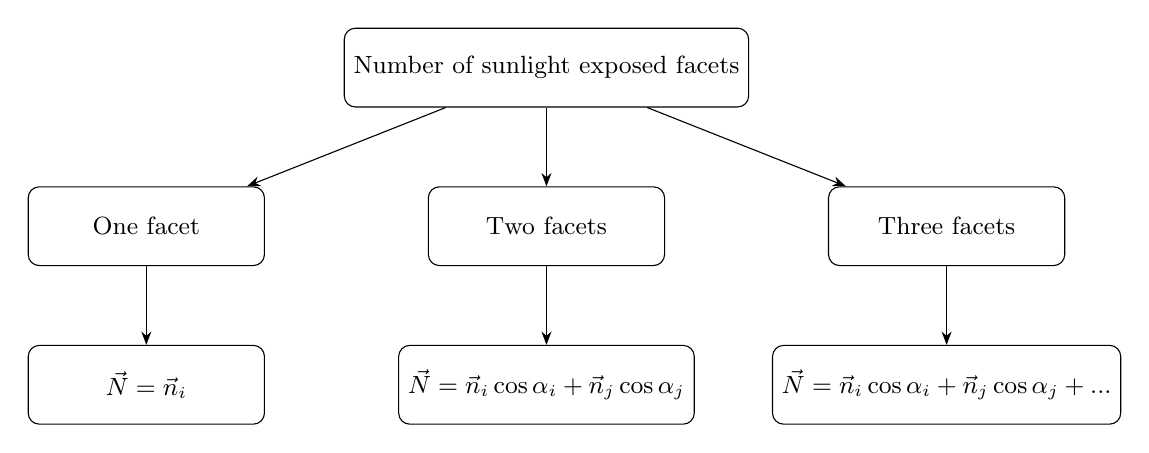
\begin{tikzpicture}[
  box/.style = {rectangle, draw, rounded corners, minimum width=3cm, minimum height=1cm, text centered, font=\small},
  >=Stealth,
  node distance=1cm and 1cm
  ]

  % Noeuds
  \node[box] (start) {Number of sunlight exposed facets};
  \node[box, below left=of start] (One facet) {One facet};
  \node[box, below=of start] (Two facets) {Two facets};
  \node[box, below right=of start] (Three facets) {Three facets};
  \node[box, below=of One facet] (1) {$\vec{N} = \vec{n}_i$};
  \node[box, below=of Two facets] (2) {$\vec{N} = \vec{n}_i \cos \alpha_i +\vec{n}_j \cos \alpha_j  $};
  \node[box, below=of Three facets] (3) {$\vec{N} = \vec{n}_i \cos \alpha_i +\vec{n}_j \cos \alpha_j  +...$};

  % Flèches
  \draw[->] (start) -- (One facet);
  \draw[->] (start) -- (Two facets);
  \draw[->] (start) -- (Three facets);
\draw[->] (One facet) -- (1);
  \draw[->] (Two facets) -- (2);
  \draw[->] (Three facets) -- (3);

\end{tikzpicture}

\vspace{1cm}
From~\eqref{eq:cos}, the Sun-Satellite vector $\vec{N}$ is given by : 
\begin{equation} \label{eq:N}
\vec{N}= \frac{\sum_{i=1}^{6} n_i I_0}{\sum_{i=1}^{6} I_i}
\end{equation}





\end{itemize}

\section{System Simulation}
In order to understand and predict the behavior of the CubeSat Attitude Determination system in real world, a matlab simulation was implemented, allowing the calculation of both the Sun-Satellite vector and the Magnetic vector which represent the attitude of the CubeSat in space, using the Aerospace toolbox.


\begin{figure}[H]  % Use [H] to place exactly here (requires the float package)
    \centering
    \includegraphics[width=0.8\textwidth]{fig/matlabSimu.png}
    \caption{System on Simulink}
    \label{fig:System on Simulink}
\end{figure}

\subsection{Magnetic system}

\begin{minipage}{0.3\textwidth}

The first part of the CubeSat Attitude Determination system is the magnetic field detection. The magnetic field sensor was simulated using the International Geomagnetic Reference Field provided by the Aerospace toolbox from Matlab. 


\end{minipage}
\hfill
\begin{minipage}{0.6\textwidth}
    \centering
    \includegraphics[width=\linewidth]{fig/magneticSys.png}
    \captionof{figure}{Magnetic system on Simulink}
    \label{fig:Magnetic system on Simulink}
\end{minipage}

\vspace{1cm}

On the December 6th, 2003, the cubeSat is situated at a \textbf{Geodetic Latitude of $80°$} and a \textbf{Geodetic Longitude of $230°$}, and it's altitude is oscillating around \textbf{500km for a low Earth orbit} -later LEO-, according to the following equation :

\begin{equation}
h = 500 + 100 \cdot \sin\left( \frac{2\pi t}{600} \right)
\end{equation}


\subsubsection{Results}

\begin{table}[h!]
\centering
\begin{tabular}{|c|c|c|c|}
\hline
\textbf{Component}&\textbf{Simulation Values (nGauss)} & \textbf{Real Values (nGauss)} & \textbf{Error (\%)} \\
\hline
Bx & 1.40e+07 & 5.00e+07 & 72 \\
\hline
By & 1.35e+07  & 1.20e+07  & 12.5 \\
\hline
Bz & 57.34e+07 & 53.00e+07 & 8.18 \\
\hline
\end{tabular}
\caption{Comparison between simulation and real values}
\end{table}
The large error observed in the x-component of the magnetic vector is due to altitude variation, as the real values are only approximations of the magnetic field at an altitude of 500 km \cite{center_ncei_nodate}.

\newpage
\subsection{Solar system}

\begin{minipage}{0.3\textwidth}
In order to determine the attitude of the CubeSat, its Sun-Satellite vector $\vec{N}$ needs to be calculated a explained ealier (see pages 9 and 10). Thus, a simulation of the solar panels response was established 


\end{minipage}
\hfill
\begin{minipage}{0.6\textwidth}
    \centering
    \includegraphics[width=\linewidth]{fig/solarSys.png}
    \captionof{figure}{Solar sensor system on Simulink}
    \label{fig:Solar sensor system on Simulink}
\end{minipage}
\vspace{1cm}
\begin{lstlisting}
function intensities = SolarPanelsResponse(sunVec, R_cubesat)

sunVec = sunVec / norm(sunVec);

sunVec_body = R_cubesat * sunVec;

normals = [ 1  0  0;   
           -1  0  0;  
            0  1  0;   
            0 -1  0;   
            0  0  1;  
            0  0 -1];  

intensities = max(0,normals * sunVec_body) ;

\end{lstlisting}
\vspace{1cm}
The sun was represented by a simple unit vector pointing to a certain direction, this vector was represented in CubeSats' frame, then 6 normal vectors in (+x, -x, +y, -y, +z, -z) were created. The dot product between the normal vector of the facet and the sun unit vector gives how much sunlight hits the facet in question.\\[0.5cm]

After the acquisition of the light intensities on each facet, the Sun-Satellite vector is calculated using equation~\eqref{eq:N} -previously explained.

\subsubsection{Results}
\begin{figure}[H]  % Use [H] to place exactly here (requires the float package)
    \centering
    \includegraphics[width=0.9\textwidth]{fig/SimuResult.png}
    \caption{Simulated Vectors Representation}
    \label{fig:Simulated Vectors Representation}
\end{figure}

\section{Future Improvements}
\begin{enumerate}
\item \textbf{Integration of Gravity Vector Estimation via Accelerometer} \\ [0.3cm]
To increase the accuracy of the CubeSat Attitude Determination system, the integration of an onboard 3-axis accelerometer is considered as a potential mprovement. By combining gravitaional data with the magnetic and solar data, more reliable and robust results can be achieved.
\end{enumerate}

\newpage

% References
\addcontentsline{toc}{section}{References}
\bibliographystyle{plain}
\bibliography{Determination_attitude}  % Create a references.bib file if needed

\end{document}

